%%%%%%%%%%%%%%%%%%%%%%%%%%%%
% CHAPTER 7 - DISCUSSION of THEORY: SUPPORTING
%%%%%%%%%%%%%%%%%%%%%%%%%%%%
%%%%%%%%%%%%%%%%%%%%%%%%%%%%%%%%%%%%%%%%%%%%%%%%%%%%%%%%%%%%%%%%%%%%%%%%%%%%%%%%%%%%%%%%%%
% Richard Boardman PhD Thesis: Improving Tool Support for Personal Information Management
%%%%%%%%%%%%%%%%%%%%%%%%%%%%%%%%%%%%%%%%%%%%%%%%%%%%%%%%%%%%%%%%%%%%%%%%%%%%%%%%%%%%%%%%%%
%%%%%%%%%%%%%%%%%%%%%%%%%%%%%%%%
% DISCUSS: relate to satisficing nature 
%%%%%%%%%%%%%%%%%%%%%%%%%%%%%%%%
% ~\cite{barreau:95} notes the \textit{satisficing} nature of PIM. However there is more at play here. It is not just a lack of time, which infers some satisficing decision as directed by efficiency constraints}
%%%%%%%%%%%%%%%%%%%%%%%%%%%%%%%%
% Supporting nature beyond satisficing: distraction, futzing, discretional
%%%%%%%%%%%%%%%%%%%%%%%%%%%%%%%%
% Also a lack of inclination, they are discretionary and may not even be necessary at all.  However in some cases the user will perform them anyway}
%%%%%%%%%%%%%%%%%%%%%%%%%%%%%%%%
% cognitive work activities
%%%%%%%%%%%%%%%%%%%%%%%%%%%%%%%%
% \textit{DISCUSS: cognitive work activities}
%%%%%%%%%%%%%%%%%%%%%%%%%%%%%%%%
% information foraging
%%%%%%%%%%%%%%%%%%%%%%%%%%%%%%%%
% Contrast with Pirolli and Card's embedding of information foraging within context of another task
%%%%%%%%%%%%%%%%%%%%%%%%%%%%%%%%
% Production tasks++
%%%%%%%%%%%%%%%%%%%%%%%%%%%%%%%%
% {Not just production tasks, also emotional needs, e.g lets keep those pictures as they are nice and maybe I will want to see them again. But also consider irrational aspects. What if no production activity?
%%%%%%%%%%%%%%%%%%%%%%%%%%%
% Link to ongoing theme
%%%%%%%%%%%%%%%%%%%%%%%%%%%
% \item Not a single goal, in fact a multiplicity of shifting short-term/long-term goals as driven by production tasks.  Need to juggle to prioritize?  \textit{How to measure user costs overall? Impact on methodology. LINK to method section below}




% \newpage
%%%%%%%%%%%%%%%%%%%%%%%%%
% SUPPORTING/REFLECTION
% Lack of reflection}
%%%%%%%%%%%%%%%%%%%%%%%%%
%%%%%%%%%%%%%%%%%%%%%%%%%%%%%%%%%%
\subsection{PIM as a Supporting Activity}
\label{discussion:supporting}
%%%%%%%%%%%%%%%%%%%%%%%%%%%%%%%%%%
% Relationship of PIM with production activities
% Provide examples of production activities
% Relationship between PIM and production activities and other supporting activities (e.g. brainstorming)
% Acceptance of problems, get worse in background (USE IN LONGIT/USER EXPERIENCE/REFLECTION)
% Paradox of the supporting tool.  Trying to improve a tool that distracts people from what they're meant to be doing! (USE IN THEORY DEV: BALANCE MODEL)
%%%%%%%%%%%%%%%%%%%%%%%%%%%%%%%%%%

%%%%%%%%%%%%%%%%%%%%%%%%%%%%%%%%
% \subsubsection{ONTO SUPPORTING}
%%%%%%%%%%%%%%%%%%%%%%%%%%%%%%%%

%%%%%%%%%%%%%%%%%%%%%%%%%
% LINK TO NEXT SECTION
%%%%%%%%%%%%%%%%%%%%%%%%%
%%%%%%%%%%%%%%%%%%%%%%%%%%%%%%%%%%%%%%%%%%%%%%%%
% Consider cross-tool supporting activities
%%%%%%%%%%%%%%%%%%%%%%%%%%%%%%%%%%%%%%%%%%%%%%%%
% FOR EXAMPLE: need for coordination. Overheads of coordinating tools together
% Cross-tool \textit{production activities} involving multiple PIM-tools, evidenced by folder overlap
%%%%%%%%%%%%%%%%%%%%%%%%%%%%%%%%%%%%%%%%%%%%%%%%%%%%%%%%%%%%%%%%%%%%%%%%%%%%%%%%%%%%%%%%%%%%%%%%%%%%%%%%%%%%%%%%%
%In many cases, multiple PIM-tools are involved in managing information in support of common production activities (\textit{Need to define production/supporting activities}).  This phenomenon is confirmed by the observations of \textit{folder overlap} in \textbf{Chapter~\ref{chapter:exploratory_study}}.  For such activities, users must also encounter overheads due to coordinating related information resources across multiple collections.
%%%%%%%%%%%%%%%%%%%%%%%%%%%%%%%%%%%%%%%%%%%%%%%%%%%%%%%%%%%%%%%%%%%%%%%%%%%%%%%%%%%%%%%%%%%%%%%%%%%%%%%%%%%%%%%%
%\textbf{Section~\ref{discussion:supporting}} discusses the relationship between PIM and the production tasks that it supports.  The section highlights that inter PIM-tool integration is particularly important when a multiple PIM-tools are involved in a particular production task.
%%%%%%%%%%%%%%%%%%%%%%%%%%%%%%%%%%%%%%%%%%%%%%%%%%%%%%%%%%%%%%%%%%%%%%%%%%%%%%%%%%%%%%%%%%%%%%%%%%%%%%%%%%%%%%%%%
%The next section moves on to consider the \textit{supporting} nature of PIM, and to discuss optimal routes for designing integration mechanisms.
%%%%%%%%%%%%%%%%%%%%%%%%%%%%%%%%%%%%%%%%%%%%%%%%%%%%%%%%%%%%%%%%%%%%%%%%%%%%%%%%%%%%%%%%%%%%%%%%%%%%%%%%%%%%%%%%%
%It is argued that current PIM-tools do not provide good support for cross-tool production activities.
%%%%%%%%%%%%%%%%%%%%%%%%%%%%%%%%%%%%%%%%%%%%%%%%%%%%%%%%%%%%%%%%%%%%%%%%%%%%%%%%%%%%%%%%%%%%%%%%%%%%%%%%%%%%%%%%%
% \textbf{Section~\ref{discussion:cross-tool}} discussed the \textit{cross-tool} nature of PIM.
% This section considers PIM from a second theoretical perspective: that of PIM as a \textit{supporting} task, one that is performed by a user in support of their production goals.
% A number of empirical findings from the studies reported in previous chapters highlight the supporting nature of PIM.
% The supporting nature of PIM is highlighted by the following quote from participant M6 in the main study reported in : . Similar paradoxical views were reported by several participants in the study: that PIM is a necessary activity, but one that is equally unimportant.
% This indicates a paradoxical situation, whereby participants were driven to manage their information, yet ran the risk of wasting time in doing so.
%%%%%%%%%%%%%%%%%%%%%%%%%%%%%%%%%%%%%%%%%%%%%%%%%%%%%%%%%%%%%%%%%%%%%%%%%%%%%%%%%%%%%%%%%%%%%%%%%%%%%%%%%%%%%%%%%
% When asked how their time could be better spent, participants typically responded that they should be doing ``real work'' rather than managing files or email.
%%%%%%%%%%%%%%%%%%%%%%%%%%%%%%%%%%%%%%%%%%%%%%%%%%%%%%%%%%%%%%%%%%%%%%%%%%%%%%%%%%%%%%%%%%%%%%%%%%%%%%%%%%%%%%%%%
% Participant F2 identified ``writing papers'' as what he should be doing rather than managing files.
% PIM was often seem as an escape or a therapeutic break from work.
% Yet users are clearly driven to carry out PIM in some form on a regular basis, if as nothing more than a break from ``real work''. % ADD QUOTE.
%%%%%%%%%%%%%%%%%%%%%%%%%%%%%%%%%%%%%%%%%%%%%%%%%%%%%%%%%%%%%%%%%%%%%%%%%%%%%%%%%%%%%%%%%%%%%%%%%%%%%%%%%%%%%%%%%
% Lack of reflection - emphasised background nature of PIM.
% lack of reflection (how tool and study in general prompted reflection).  
% The longitudinal study also highlighted the \textit{lack of attention} many users devote to PIM.  
%%%%%%%%%%%%%%%%%%%%%%%%%%%%%%%
% PROMOTION OF REFLECTION
%%%%%%%%%%%%%%%%%%%%%%%%%%%%%%%
% Participants suggested that both the study and tool interventions increased
% the amount of time they devoted to reflecting on PIM. 
% \textit{Self-auditing effect:	Need to delete that, that's where that is}
% All participants in the main study indicated that their participation, combined with the design intervention, lead them to devote more attention to PIM.  For example, during the interviews many participants performed tidying of their file, email and bookmark collections -- the interviews had a clear ``self-auditing'' effect.
%%%%%%%%%%%%%%%%%%%%%%%%%%%%%%%%%%%%%%%%%%%%%%%%%%%%%%%%%%%%%%%%%%%%%%%%%%%%%%%%%%%%%%%%%%%%%%%%%%%%%%%%%%%%%%%%%
%%%%%%%%%%%%%%%%%%%%%%%%%%%%%%%%%%%%%%%%%%%%%%%%%%%%%%%%%%%%%%%%%%%%%%%%%%%%%%%%%%%%%%%%%%%%%%%%%%%%%%%%%%%%%%%%%
%%%%%%%%%%%%%%%%%%%%%%%%%%%%%%%%%%%%%%%%%%%%%%%%%%%%%%%%%%%%%%%%%%%%%%%%%%%%%%%%%%%%%%%%%%%%%%%%%%%%%%%%%%%%%%%%%
%%%%%%%%%%%%%%%%%%%%%%%%%%%%%%%%%%%%%%%%%%%%%%%%%%%%%%%%%%%%%%%%%%%%%%%%%%%%%%%%%%%%%%%%%%%%%%%%%%%%%%%%%%%%%%%%%

%%%%%%%%%%%%%%%%%%%%%%%%%%%
% \subsubsection{Evidence for this view}
%%%%%%%%%%%%%%%%%%%%%%%%%%%%%%%%
% FOUNDATION: supporting data
%%%%%%%%%%%%%%%%%%%%%%%%%%%%%%%%
% The author developed this view during the empirical work reported in \textbf{Chapters~\ref{chapter:exploratory_study}} and \textbf{\ref{chapter:main-study}}.
In both studies participants reported that the interviews caused them to spend a lot more time thinking about PIM than normal.  Although they carried out PIM everyday, PIM was not an activity that most reported spending time focused on.  In the main study, when asked about their PIM practices regarding files, email and bookmarks, PIM was portrayed as a necessary activity, yet one that was not considered to be ``real work'' (see \textbf{Section~\ref{main-study:results:reflection}}).  In fact, a number of participants saw PIM as a chance for a welcome break, or as a waste of time! %, \textit{M6: ``There is never enough time to do PIM, and whatever time you do spend on it is often wasted''}.

%%%%%%%%%%%%%%%%%%%%%%%%%%%%%%%%%%%%%%%%%%%%%%%%
% ARGUE THAT PIM IS SUPPORTING BASED ON THIS
% Instead users are focused on production goals.  
%%%%%%%%%%%%%%%%%%%%%%%%%%%%%%%%%%%%%%%%%%%%%%%%
These results support the conceptualization of PIM as a \textit{supporting} activity.  This section suggests that it is a user's high-level production activities and goals, their ``real work'', that provide direction to their otherwise discretionary PIM activity.  The next section extends the theoretical framework from \textbf{Section~\ref{discussion:cross-tool}} to encompass this view.

%%%%%%%%%%%%%%%%%%%%%%%%%%%%%%%%%%%%%%%%%%%%%%%%%%%%%%%%%%%%%%%%%%%%%%%%%%%%%%%%%%%%%%%%%%%%%%%%%%%%%%%%%%%%%%%%%
%%%%%%%%%%%%%%%%%%%%%%%%%%%%%%%%%%%%%%%%%%%%%%%%%%%%%%%%%%%%%%%%%%%%%%%%%%%%%%%%%%%%%%%%%%%%%%%%%%%%%%%%%%%%%%%%%
%%%%%%%%%%%%%%%%%%%%%%%%%%%%%%%%%%%%%%%%%%%%%%%%%%%%%%%%%%%%%%%%%%%%%%%%%%%%%%%%%%%%%%%%%%%%%%%%%%%%%%%%%%%%%%%%%
%%%%%%%%%%%%%%%%%%%%%%%%%%%%%%%%%%%%%%%%%%%%%%%%%%%%%%%%%%%%%%%%%%%%%%%%%%%%%%%%%%%%%%%%%%%%%%%%%%%%%%%%%%%%%%%%%
% The next section extends the theoretical framework proposed \textbf{Section~\ref{discussion:cross-tool}} to describe this relationship.

%%%%%%%%%%%%%%%%%%%%%%%%%%%%%%%%%
\subsubsection{Production and Supporting Activities}
%%%%%%%%%%%%%%%%%%%%%%%%%%%%%%%%%
% Finally, the study highlighted the supporting nature of PIM. Here, several avenues are suggested for modifying the framework to capture the influence of an individual's production tasks in determining their PIM needs.
% In this section, a theoretical framework is developed to differentiate PIM and the production activities it supports.
Based on the above discussion, two types of activity are introduced:

\begin{enumerate}

%%%%%%%%%%%%%%%%%%%%%%%%%%%%%%%%%%%
% Define production activities
%%%%%%%%%%%%%%%%%%%%%%%%%%%%%%%%%%%
\item \textit{Production activities} are defined as the ``high-level'' work and leisure activities which drive a user's computer usage.  In a work context, these are the activities on which the user's performance is appraised. For example, a lawyer's production activities may include presenting court cases and writing wills for clients.  For a student, production activities may include completing coursework and revising for exams.

%%%%%%%%%%%%%%%%%%%%%%%%%%%%%%%%%%%%
% Define supporting activities
%%%%%%%%%%%%%%%%%%%%%%%%%%%%%%%%%%%%
% Must be careful - more to PIM drive than production task
\item \textit{Supporting activities} are performed to promote the completion of production activities.  In other words, they are not carried out for their own sake, instead they are ``the things one does to get something else done''.  PIM, the focus of this thesis, is a key supporting activity.  It is argued that PIM is not the primary reason people use computers.  Instead, it is performed to support their production activities.

\end{enumerate}

%%%%%%%%%%%%%%%%%%%%%%%%%%%%%%%%%%%%%%
% SUPPORTING ACTIVITIES IN GENERAL
%%%%%%%%%%%%%%%%%%%%%%%%%%%%%%%%%%%%%%
% There may be a hierarchy of production/supporting relationships
% This thesis focuses on personal information management as one supporting activity, but there are clearly many others.
% The relationship between the supporting activities involved in the example production activity of writing a report is  illustrated in
Production activities may involve multiple supporting activities.  \textbf{Figure~\ref{fig:design:PIM-production-rship-multsupp}} illustrates the supporting activities driven by an example production activity, that of writing a confidential report. These include the management of files, email, and bookmarks, communication with colleagues, updating software applications, and effective IT security practice (e.g. choosing a good password, and locking the screen).  % WHERE TO PLACE: DISCUSS DISCRETIONARY IN DEPTH
There may also be a nested arrangement of production/supporting relationships.  For example, email-based PIM can be seen as an activity that supports collaboration with co-authors, which in turn supports the overall production goal of writing the report.

In a work context, some supporting activities, such as security awareness may be enforced through guidelines.  The others shown in \textbf{Figure~\ref{fig:design:PIM-production-rship-multsupp}}, including PIM, are important, but \textit{discretionary}. Typically, the employee is not directly appraised regarding their execution. In fact, PIM is often the personal responsibility of the employee who can choose whether and to what extent they perform it.  This \textit{discretionary} nature of PIM has both positive and negative consequences.  Users are given the freedom to manage information as they choose, and may well have strong views about how to do so.  However, users typically receive little help from employers regarding the problems they encounter.





% %%%%%%%%%%%%%%%%%%%%%%%%%%%%%
% FIGURE - Relationship between supporting activities and production activities
% %%%%%%%%%%%%%%%%%%%%%%%%%%%%%
%%%%%%%%%%%%%%%%%%%%%%%%%%%%%%
\begin{figure}[htbp]
	\begin{center}
		\leavevmode
		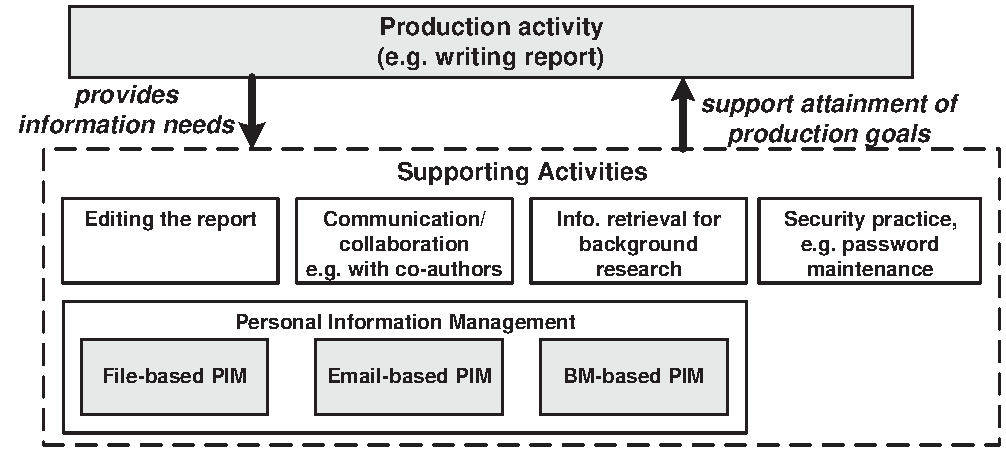
\includegraphics[height=6cm]{pictures/discussion/PIM-production-rship-multsupp.pdf}
		% fs-fm-comparison.pdf}
	\end{center}
	\caption{Supporting activities involved in the production activity of writing a report}
	\label{fig:design:PIM-production-rship-multsupp}
\end{figure}

%%%%%%%%%%%%%%%%%%%%%%%%%%%%%%%%%
% CONTRAST WITH WORK/ENABLING
%%%%%%%%%%%%%%%%%%%%%%%%%%%%%%%%%
The production/supporting relationship can be contrasted with a previous conceptualization of \textit{work} and \textit{enabling} tasks~\citep{Whitefield:93}.  Enabling tasks are tasks that are \textit{required to achieve a work goal}. For example, the enabling task of ``pressing a key'' helps achieve the work goal of ``typing a sentence in a report''.  In contrast, the supporting activities outlined above are secondary, but \textit{discretionary}.  Furthermore, \citet{Whitefield:93} focus on lower-level tasks than those discussed here. In contrast, all the example supporting activities in \textbf{Figure~\ref{fig:design:PIM-production-rship-multsupp}} are ongoing high-level activities.  



%%%%%%%%%%%%%%%%%%%%%%%%%%%%%%%%%%%%%%%%%%%%%%%%%%%%%
\subsubsection{Extending the Theoretical Framework}
%%%%%%%%%%%%%%%%%%%%%%%%%%%%%%%%%%%%%%%%%%%%%%%%%%%%%

%%%%%%%%%%%%%%%%%%%%%%%%%%%%%%%%%%
% SIMPLIFY WITH A FOCUS ON PIM
%%%%%%%%%%%%%%%%%%%%%%%%%%%%%%%%%%
% For example, the management of files requires some need to manage the data in those files.  
% Multiple supporting acytivities are beyond scope of the thesis -- only some simple examples are considered here.
% Here a focus is taken on PIM as a stand-alone supporting activity. 
\textbf{Figure~\ref{fig:design:PIM-production-simple}} extends the framework from the previous section to accommodate the relationship between PIM as a \textit{cross-tool, supporting activity} and a user's production activities.  Production activities provide the information needs which drive PIM\footnote{A similar idea is common in the information retrieval literature whereby an external need drives a user's information seeking~\citep{wilson:00}.}. PIM offers support for the production activity by supplying information resources and reminders.
% A user's production activities supply the information needs which in turn drive the need to perform PIM.  

% %%%%%%%%%%%%%%%%%%%%%%%%%%%%%
% FIGURE - SIMPLE Relationship between PIM and production activities
% %%%%%%%%%%%%%%%%%%%%%%%%%%%%%
%%%%%%%%%%%%%%%%%%%%%%%%%%%%%%
\begin{figure}[htbp]
	\begin{center}
		\leavevmode
		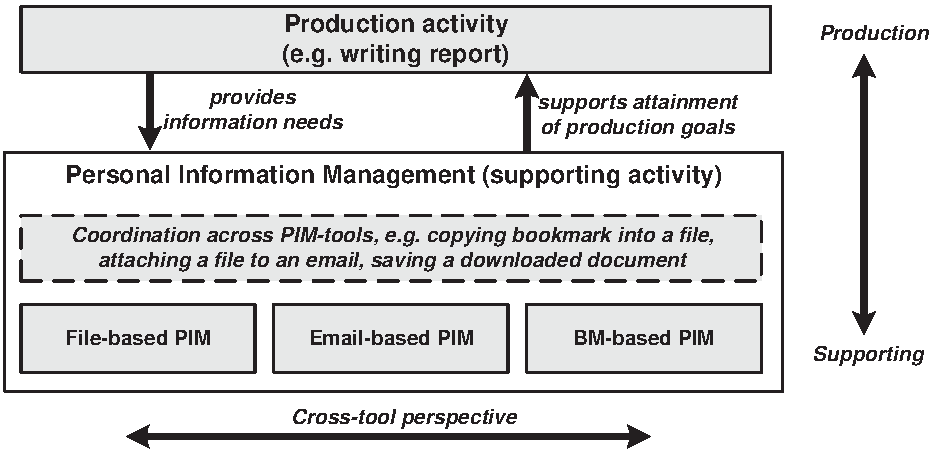
\includegraphics[height=6cm]{pictures/discussion/PIM-production-rship-pimfocus.pdf}
		% fs-fm-comparison.pdf}
	\end{center}
	\caption{Theoretical framework extended to reflect the cross-tool, supporting nature of PIM}
	\label{fig:design:PIM-production-simple}
\end{figure}


%%%%%%%%%%%%%%%%%%%%%%%%%%%%%%%%%%%%%%%%%%%%%
% MAPPING FROM PIM-TOOLS TO PRODUCTION TASKS
%%%%%%%%%%%%%%%%%%%%%%%%%%%%%%%%%%%%%%%%%%%%%
%%%%%%%%%%%%%%%%%%%%%%%%%%%%%%%%%%%%%%%%%%%%%%%%%%%%%%%%%%%%%%%%%%%%%%%%%%%%%%%%%%%%%%%%%%%%%5
% Note that not a simple mapping. Actually, many-many between PIM-tools and production tasks.
%%%%%%%%%%%%%%%%%%%%%%%%%%%%%%%%%%%%%%%%%%%%%%%%%%%%%%%%%%%%%%%%%%%%%%%%%%%%%%%%%%%%%%%%%%%%%%
% But note: not simply so, see production activities below -- have to relate to multiple strategies/multiple production activities. Some are cross-tool, some are not. However, it is not a simple mapping from PIM-tools to production activities.
% Actually, many-many between PIM-tools and production tasks.
% There is a many-many mapping between PIM-systems and production activities. % In other words, production activities vary in terms of how many PIM-tools are involved in supporting them.  
Two types of production activity can be identified in terms of the number of PIM-tools which support them:

\begin{enumerate}

\item Some production activities are \textit{tool-specific} -- they only involve PIM activity within the bounds of one PIM-tool.  A simple example of a tool-specific production activity is offered: arranging a picnic with friends. This involves the exchange of emails with friends, and their storage.  At a later time, the received messages are consulted to edit a reminder to coordinate who is bringing what food and drink.  The PIM needs for this task are email-specific.  Tool-specific production activities do not require integration support.
%%%%%%%%%%%%%%%%%%%%%%%%%%%%%%%%%%%%%%%%%%%%%%%%%%%%%%%%%%%%%%%%%
% Different PIM-tools have different \textit{raison d'etres}? 
% Core functions. This is a different slicing of activity space
%%%%%%%%%%%%%%%%%%%%%%%%%%%%%%%%%%%%%%%%%%%%%%%%%%%%%%%%%%%%%%%%%
% Email tools can be considered to be PIM tool that primarily supports the communication needs of production tasks.  Likewise, bookmark tools are a PIM-tool that primarily supports the information retrieval needs of production tasks.  Thus production activities focused on one of these aspects (e.g. book flight) may naturally be limited to one PIM-tool.

%%%%%%%%%%%%%%%%%%%%%%%%%%%%%%%%%%%%%%%%%%%%%%%%%%%%%%%%%%%%%%%%%%%%%%%%%%%%%%%
% Discuss: ONE PRODUCTION TASK/MANY PIM-tools
% Some cross-tool production tasks may be centered on particular PIM-tools.
%%%%%%%%%%%%%%%%%%%%%%%%%%%%%%%%%%%%%%%%%%%%%%%%%%%%%%%%%%%%%%%%%%%%%%%%%%%%%%%
% NB: different tools can act as gateway into a cross-tool task
%%%%%%%%%%%%%%%%%%%%%%%%%%%%%%%%%%%%%%%%%%%%%%%%%%%%%%%%%%%%%%%%%%%%%%%%%%%%%%%
% True cross-tool tasks (with primary tools?)
% Tool-dominated tasks which involved "`excusrsions"' to other tools
% Some production activities are distributed.
% \textbf{Section~\ref{discussion:cross-tool}} introduces the notion of PIM as a cross-tool activity, one that bridges multiple tools.  Some production tasks may require support from multiple PIM-tool contexts.  Provide benchmark cross-tool production tasks: Nice example. Show how it necessitates \textbf{coordination} of sub-activities and tools towards a common goal. Example cross-tool production task,e.g. more organizational needs in one tool: ISIS (may still be tool-driven). 
\item Other production activities are \textit{cross-tool} -- they involve the management of information in multiple PIM-tools.  For example, planning a holiday may involve collating websites, sending and storing emails, and creating files with possible itineraries.
%
%%%%%%%%%%%%%%%%%%%%%%%%%%%%%%%%%%
% RELATE TO INTEGRATION MECHANISMS
%%%%%%%%%%%%%%%%%%%%%%%%%%%%%%%%%%%
When production activities involve multiple PIM tools, there is the need for \textit{coordination} between those PIM-tools.  This may be as simple as transferring a bookmark from a web browser to include in an email message.  Alternatively, coordination may be more extensive, e.g. the ongoing management of emails and bookmarks relating to a long-term project. 
% Show how ONE-MANY necessitates \textbf{coordination} of sub-activities and tools towards a common goal. 
% Such production tasks that require cross-tool PIM support, may necessitate coordination of PIM activity across multiple tools.  
% Another example would be retrieving a holiday itinerary, when the user is not sure if it is stored in the file system, or as an email attachment. Other coordination examples include starting or finishing a project that involves multiple PIM tools.
%%%%%%%%%%%%%%%%%%%%%%%%%%%%%%%%%%%%%
% Discuss integration as designed-in coordination, alternative is manual coordination
% Where does integration fit in?
%%%%%%%%%%%%%%%%%%%%%%%%%%%%%%%%%%%%
% Certain production activities involve the coordination of multiple PIM-tools.  Integration mechanisms between PIM-tools can help support such coordination activities.
\textit{Integration mechanisms} can be viewed as interface functionality which support cross-tool coordinating activities, thus avoiding the need for manual coordination. By making it easier to coordinate information requirements across multiple PIM-tools, the overheads of manual coordination are lessened.
% In particular, the importance of integration between the PIM-tools involved in cross-tool production activities is noted. 
% Integration mechanisms can relieve users of some of the burden of performing coordination activities.  For example, the Windows ``Send-to'' mechanism allows bookmarks to be sent directly as email messages.

\end{enumerate}

%%%%%%%%%%%%%%%%%%%%%%%%%%%%%%%%%%%%%%%%%%%%%%%%%%%%%%%%%%%%%%%%%%%%
% \subsubsection{A final note on PIM as a supporting activity}
%%%%%%%%%%%%%%%%%%%%%%%%%%%%%%%%%%%%%%%%%%%%%%%%%%%%%%%%%%%%%%%%%%%%


% It is argued that much of the literature focuses on PIM as a production ``work'' task.  
% WHERE TO PLACE: DISCUSS INTERFERENCE WITH PRODUCTION TASKS + LIBRARIAN
This section has discussed how PIM is not a self-contained, stand-alone activity, but one that is driven by a user's production activities.  However, note that information management can itself be a production activity.  For example, consider how librarians manage information for others as one of their key job responsibilities.

% In contrast, PIM is conceptualized here as a supporting activity, one that is driven by the information needs provided by a user's production tasks\footnote{Note that some aspects of PIM may be considered as a self-contained production task by some, e.g. maintenance.}.
The relationship between PIM as a supporting activity, and a user's production activities also illustrates the distraction that PIM can cause.  At times, PIM may interfere with a user's production activities by consuming all of a user's attention.  For example, consider the situation when a user is unable to find a very important document and devotes an entire morning to finding it. In this case, PIM may displace the goals corresponding to the ``real'' production activity. \textbf{Section~\ref{discussion:uxp}} discusses the methodological implications caused by the potential of PIM to cause such distraction: do PIM designers run the risk of encouraging users to spend less time on their production activities?





%%%%%%%%%%%%%%%%%%%%%%
% LINK TO THEORY
%%%%%%%%%%%%%%%%%%%%%%
% \textit{Include links to design and theory-building}
%%%%%%%%%%%%%%%%%%%%%%%%%%%%%%%%
% LINK TO BALANCE SECTION
%%%%%%%%%%%%%%%%%%%%%%%%%%%%%%%%
% Relate to models developed in \textbf{Section~\ref{disc:study-discussion}} in terms of the ``need for balance'' (user needs to do enough PIM to support production activities, but not too much to become distracted). 
% Also relate to design ideas in \textbf{Section~\ref{disc:design-guidelines-discussion}}.
% Pros and cons of discretional supporting activity
% Potential for interference, impact on productivity on upside and downside.  Therefore need for balance.  Lead onto the next section.
%%%%%%%%%%%%%%%%%%%%%%%%%%%%%%%%%%%%%
% LINK - develop user experience
%%%%%%%%%%%%%%%%%%%%%%%%%%%%%%%%%%%%%
% Furthermore, it is these high-level activities that distract their attention from PIM.}


%%%%%%%%%%%%%%%%%%%%%%%%%%%%%%%%%%%%%%%%%%%%%%%%%%%%%%%%%%%%%%%%%%%%%%%%%%%%%%%%%%%%%%%%%%%%%%%%%%%%%%%%%%%%%%%%%
%%%%%%%%%%%%%%%%%%%%%%%%%%%%%%%%%%%%%%%%%%%%%%%%%%%%%%%%%%%%%%%%%%%%%%%%%%%%%%%%%%%%%%%%%%%%%%%%%%%%%%%%%%%%%%%%%
%%%%%%%%%%%%%%%%%%%%%%%%%%%%%%%%%%%%%%%%%%%%%%%%%%%%%%%%%%%%%%%%%%%%%%%%%%%%%%%%%%%%%%%%%%%%%%%%%%%%%%%%%%%%%%%%%
%%%%%%%%%%%%%%%%%%%%%%%%%%%%%%%%%%%%%%%%%%%%%%%%%%%%%%%%%%%%%%%%%%%%%%%%%%%%%%%%%%%%%%%%%%%%%%%%%%%%%%%%%%%%%%%%%



%%%%%%%
% FIN
%%%%%%%